\chapter{Problem\'atica de la Identificaci\'on de Filamentos a partir de un Grafo}
\label{chap:cap2}

%problema previo, o problema 0 que consiste en la generaci\'on de un grafo a partir de una imagen que contenga una red, que en este caso, representaria a una red de filamentos. 

En base lo expuesto en el cap\'itulo \ref{chap:stateoftheart}, para el enfoque de utilizar grafos para la individualizaci\'on de filamentos existe una brecha entre la obtenci\'on del grafo y su an\'alisis. Esta paso previo, la extracci\'on de un grafo a partir de una imagen, lo denominamos como el problema previo o problema 0 y consiste en extraer un grafo $G = (V,E)$ de una imagen tal que $G$ sea un grafo simple, no dirigido, ponderado, conectado o desconectado, con o sin ciclos. Esto implica que exista a lo m\'as 1 arista por cada par de nodos adyacentes, prohibi\'endose la existencia de nodos conectados consigo mismos. Se definen los v\'ertices/nodos del grafo $G$ como $V(G)$ y las aristas de $G$ como $E(G)$. 
Que el grafo $G$ sea ponderado se puede definir en $\forall e \in E(G)  \exists $ caracter\'isticas asociadas que se expresan como caracter\'isticas geom\'etricas, topol\'ogicas, espaciales y/u otras. Es importante evitar que $G$ sea un grafo completo, dado que con n nodos/v\'ertices $G$ tenga $\frac{n(n-1)}{2}$ aristas. 

Algunas de las dificultades involucradas en la extracci\'on de informaci\'on a partir de una imagen se encuentran en los m\'etodos presentados en el cap\'itulo \ref{chap:stateoftheart}, dentro de las que destacan el ruido y la resoluci\'on.

\begin{figure*}[h]
    \label{fig:NoConsenso}
    \begin{tabular}{c c c}
        \multirow[c]{2}{*}[2.5cm]{
        \begin{subfigure}[t]{0.4\textwidth}
        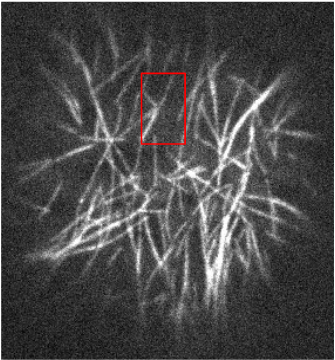
\includegraphics[scale=0.5]{imagenes/NoConsenso.png}
        \caption{Microt\'ubulos en planta {\it Marchantia}.\\Fuente: Paula Llanos}
        \label{fig:NoConsensoGeneral}
        \end{subfigure}  
        }
        &
        \multirow[c]{2}{*}[2cm]{
        \begin{subfigure}[t]{0.25\textwidth}
        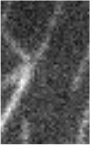
\includegraphics[]{imagenes/NoConsenso2.png}
        \caption{Secci\'on resaltada en rojo de \ref{fig:NoConsensoGeneral}}
        \label{fig:NoConsensoRect}
        \end{subfigure}
        }
        &
        \begin{subfigure}[t]{0.21\textwidth}
        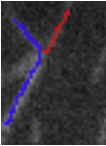
\includegraphics[scale=0.8]{imagenes/NoConsenso3.png}
        \caption{Opci\'on 1 de microt\'ubulos en \ref{fig:NoConsensoRect}}
        \label{fig:NoConsensoOpcion1}
        \end{subfigure} \\
        & &
        \begin{subfigure}[b]{0.21\textwidth}
        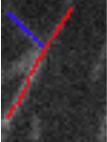
\includegraphics[scale=0.8]{imagenes/NoConsenso4.png}
        \caption{Opci\'on 2 de microt\'ubulos en \ref{fig:NoConsensoRect}}
        \label{fig:NoConsensoOpcion2}
        \end{subfigure} \\
    \end{tabular}{}
    
    \caption{Dificultad de individualizaci\'on que enfretan los expertos al analizar manualmente una imagen de filamentos, en particular, microt\'ubulos.}
\end{figure*}


Una vez obtenido el grafo que representa una red de filamentos, el problema siguiente se encuentra en el que 2 expertos pueden discernir con respecto a los filamentos identificables en una imagen, por lo que no es posible conocer a priori del origen y el final de un filamento, para las resoluciones actuales de las imagenes obtenidas a partir de la microscop\'ia. Se añade como dificultad que dada la representaci\'on de un filamento en un grafo es en base a un conjuntos de aristas adyacentes (denominadas caminos), esto puede significar la b\'usqueda en un universo de hasta $n!$ posibles combinaciones.

A partir del problema anterior, el problema final lo constituye la elecci\'on del subconjunto de caminos, que debe ser seleccionado entre el total de caminos que representan soluciones factibles. Esto implica que el problema no solo sea un problema combinatorial de generar soluciones factibles a partir del conjunto de aristas, sino que adem\'as debe considerar la discriminaci\'on entre estos para obtener el subconjunto de mayor calidad, pudiendo representarse como un problema de optimizaci\'on combinatorial.

Los 3 problemas presentados se formalizan a continuaci\'on.

%problema previo
\section{Generaci\'on de un Grafo desde una Imagen}
La extraci\'on o generaci\'on de un grafo que representa una red de filamentos a partir de una imagen es el paso que define la cantidad de informaci\'on disponible para llevar a cabo la individualizaci\'on de filamentos. La importancia de este procedimiento radica en que a partir de la imagen es posible obtener una cantidad de caracter\'isticas de distinta \'indole, lo que permite desagregar el grafo $G$ en subgrafos, siendo la primera forma de disminuir el espacio de b\'usqueda.. 


presentar el problema previo, como un puente necesario en la 
automatizaci\'on de la extracci\'on,  para analizar un grafo que representa la red de filamentos, que de lo contrario tendria que ser realizado a mano, implicando que la persona realizando el análisis podría llevar a cabo la individualizaci\'on de filamentos en el mismo acto.

Es posible distinguir en 2 conjuntos los m\'etodos utilizados para extraer la informaci\'on escencial que permite la construcci\'on de un grafo a partir de una imagen, como lo son los nodos y las aristas. Estos conjuntos son los que se basan en esqueletonizaci\'on\cite{lavado2018comparacion} y los que no. En este trabajo se presenta un enfoque del segundo tipo.

\subsection{Generador Aproximado de Grafos a partir de una Imagen}
% explicar que el hecho de G completo mediante lo q la arista es al problema de identificación de filamentos
presento el extractor aproximado de grafos, la noción de puntos cluster/superPixels/blobs y el centro de masa como representante, dado que se puede obtener de forma simple mediante los "image moments". Además, distintos niveles de image moments permiten obtener información adicional útil en la descripción del cluster.

La noción ppal es generar vecindarios, ya que el grafo debe contener información topológica como geométrica, ya que cada será la base para distintos criterios de categorización durante el proceso de individualización de filamentos. 

opcional: Un ejemplo de aquello pueden ser los ciclos, ya que con el grado de los nodos se puede determinar aquello (fuente: wilkisongraphbook)

Veselness: Se estudió el filtro Frangi para "Veselness" (fuente: frangi1998, frangiNet) utilizados para filtrar estructuras alargadas, como lo son arterias y venas. Este filtro se basa en la matriz Hessiana, y sus eigenvectores y eigenvalores para ponderar el "veselness value" (agregar formulas), 2nd order structurness, y $R_b$ blobness measure...

Dado que se puede llegar a algo similar mediante los image momentos ....

se analizaron filtros como Gabor Gaussian kernels siendo descartados ya que pierden detalles mediante el blurring (fuente: A coronary artery segmentation method based on multiscale analysis and region growing 2015). Por otra parte, el filtro  anistropic Difusion fue descartado por requerir de múltiples parámetros. 
Lo anterior se destaca ya que dentro de los criterios del generador aproximado de grafos a partir de una imagen se busca evitar perder información de la imagen, así como tener un costo computacional bajo, en conjunto con disminuir la interacción del usuario. 

numero de nodos depende de apMaxThickness, q representa la resoluci\'on, es decir, cuantos micrometros se observan por pixel.

finalmente Generaci\'on de Aristas se realiza mediante la uni\'on nodos, obtener informaci\'on angular, trabajo a futuro ser\'ia agregar curvatura 

\subsubsection{Heurística para limitar el n\'umero de nodos}
Un grafo completamente conectado puede tener n(n-1)/2 aristas, lo que para un n muy grande puede implicar un costo computacional se aplicó como estrategía: 
Node Pruning: parametro apMaxThickness y connectivityThreshold manuales. Arbitrariamente n\textdegree neighbors > 2. también se fija un límite de memoria ram


\section{Generaci\'on de Caminos}
definir que los segmentos/caminos/path son conjuntos de aristas adyacentes conectadas, o de nodos ..., que cumplen con restricciones, como la restricción angular o restricciones de ciclos (formula matem\'atica) y que los filamento son elegidos entre los caminos de mayor calidad
Un camino simple es equivalente a un \'arbol simple, ac\'clico...


En un grafo con n aristas, en el cual se desconoce el origen y el final los caminos, el n\'umero de combinaciones crece exponencialmente (agregar \cite{101 y 102 de define}). Denominamos todas estas opciones de caminos como el conjunto $P$, del cual debemos extraer un subconjunto $P'$ mediante una estrategia que permita realizar esto en tiempo polinomial independientemente de la cantidad de aristas del grafo.

\begin{equation}
p = (e_1, e_2,..., e_n)\\
p = ((v_1,v_2), (v_2,v_4),..., (v_n-1,v_n))
\label{eq:path}
\end{equation}

% explicar define
El m\'etodo presentado en \cite{breuer2015define} se basa en lo definido por \cite{lin2006vertex}, indicando que dado un problema de {\it covering}, existe un {\it set system}$(S,C)$, donde S es el conjunto total y finito de sets, y C es un conjunto de subsets pertenecientes a S. En el caso espec\'ifico del {\it Minimum Set Cover}(SC), el objetivo es encontrar un subconjunto $C'$ de $C$ tal que cada elemento de $S$ pertenezca al menos 1 vez a uno de los miembros de $C'$.

Para un {\it set system}$(S,C)$ que pueda ser representando por un \'arbol $T$, es posible modificar la definici\'on de $S$ al conjunto de nodos que componen un grafo $G$ y que cada subset $c \in C$ representa un camino\eqref{eq:path} simple en $G$. Se destaca que no necesariamente estar\'an todos los caminos simples de $G$ est\'an representados en $C$. Esta representaci\'on de {\it covering} de caminos, o {\it Path Cover}, es denominada {\it Vertex Covering by Paths on Graphs}(VcpG) y difiere de un {\it Path Cover} tradicional al permitir caminos que compartan nodos. Luego, para el caso de \'arboles, VcpG se renombra a VcpT ({\it Vertex Covering by Paths on Trees}), y si se reemplazan los nodos por aristas, lo no genera cambios significativos en el planteamiento del problema, se denomina EcpT {\it Edge Covering by Paths on Trees}. %recordar mas adelante como posible perdida de soluciones factibles


Lo anterior establece las bases para que los autores de DeFiNe\cite{breuer2015define} utilicen EcpT como base, teniendo un m\'aximo de caminos $n(n)-1/2 = \mathcal{O}(n^{2})$, con una complejidad $\mathcal{O}(n^{4})$ para obtener esos caminos, para caminos que no comparten nodos o aristas, es decir, no se sobrelapan.

La obtenci\'on de caminos a partir de un \'arbol $T$ que representa un grafo $G$ se realiza mediante la divisi\'on continua del \'arbol en m\'ultiples bosques, hasta que los bosques resultantes sean s\'olo caminos simples.

%aca entran las formas de obtener esos arboles simples y bosques, con las heuristicas de define
...


% Comparándose con define,
el problema acá está en la generación de P' subconjunto de P (caminos totales) , ya que al usar una sola propiedad, como lo puede ser el ángulo entre aristas, el largo o el ancho, se pierden soluciones. Ejemplo camino verde en Spinning Marchantia (imagenes)

% Heurística: hay alguna aca? pareciera solo satisfacci\'on de restricciones
% garantizar que al satisfacer las restricciones los caminos son solo soluciones factibles y que la unión de caminos también entrega múltiples opciones de filamentos, los que deben ser medidos para determinar cual es mejor




\section{Modelo de Optimización}
%dado que se tienen muchos filamentos, se debe evaluar cual es mejor. Explicar como propiedades topológicas y geométricas tienen. Y como se ponderan para un peso que será minimizado o maximizado

En base a lo recopilado en las secciones previas de esta investigaci\'on, es posible destacar los siguientes aspectos al problema a resolver:

\begin{itemize}
    \item Se desconoce a priori el n\'umero de filamentos a buscar, dado que una imagen puede tener individualizaciones distintas para 2 expertos.
    \item Generalmente, se busca individualizar m\'as de un filamento por imagen, lo que conlleva a elegir los mejores filamentos entre las soluciones que se encuentren.
    \item El uso de un grafo para representar la red de filamentos puede implicar que las combinaciones de soluciones crezca de manera exponencial.
\end{itemize}

Lo anterior implica que el problema de identificar filamentos a partir de un grafo puede ser clasificado como un problema de optimizaci\'on de restricciones\cite{blum2011hybrid}.

Un problema de optimización de restricciones, (COP por su sigla en ingl\'es) puede ser representado como $P = (S, \Omega, F)$, donde S es el espacio de soluciones, definido por un conjunto discreto de variables $X = 1 \dotsc n$, con valores $v_{i}^{j} \in D_{i} = \{v_{i}^{1} \dotsc  v_{i}^{|D_{i}|}\}$. Se define como una variable {\it instanciada} la asignaci\'on a $X_i$ de un valor $v_{i}^{j} \in D_i$. Una solución candidata $s \in S$, es una soluci\'on factible si satisface las restricciones del set $\Omega$. La funci\'on objetivo $F: S\rightarrow \mathbb R_{0}^{+}$, es la funci\'on de evaluaci\'on que asigna valores a las soluciones candidatas. Por su parte, $s^{*} \in S^{*} \subseteq S $, $c$ es una soluci\'on \'optima y $S^{*}$ es un conjunto de soluciones \'optimas\cite{socha2008ant}.
Esta definici\'on permite aplicar la metaheur\'istica de optimizaci\'on basada en colonia de hormigas (ACO por su sigla en ingl\'es) a un modelo de un {\it COP}.
%COP es un CSP con función objetivo: https://en.wikipedia.org/wiki/Constrained_optimization#Constraint_optimization_problems

\subsection{Metaheur\'istica ACO}
El proposito de la metaheur\'istica ACO es encontrar una soluci\'on o un set de soluciones. Una soluci\'on $s$ consiste en un conjunto de componentes de soluci\'on $c_{ij} \in C, i = 1 \dotsc n, j = 1 \dotsc |D_i|$, por lo que una concatenaci\'on de componentes de soluci\'on forma el camino o {\it tour} que recorre una hormiga, desde un nodo o arista inicial hasta un nodo o arista final. La metaheur\'istica ACO se muestra en el algoritmo \ref{ACO-Algo}. En base a la definici\'on de variable {\it instanciada} del modelo COP, se tiene que $X_i = v_{i}^{j}$ es el equivalente a $c_{ij}$ en ACO.

ACO consiste en un paso de inicializaci\'on y de tres componentes, las que no tienen un orden espec\'ifico: {\it Construccion\_de\_soluci\'on\_de\_cada\_hormiga(),  M\'etodo\_de\_b\'usqueda\_no\_local()} y {\it Actualizaci\'on\_de\_feromonas()}.


\begin{algorithm}[H]
\SetAlgoLined
\KwData{Variables $X_i \dotsc X_n$, dominios $D_1 \dotsc D_n$, Restricciones $\in \Omega$}
\KwResult{conjunto s\textquotesingle $ \subseteq S$ != $\emptyset$, si existen soluciones factibles}
 Ajuste de Par\'ametros \& inicializaci\'on de feromonas \;
 \While{Criterio de finalización no se cumple}{
   Planificaci\'on\_de\_Pasos\;{
   ~ Construccion\_de\_soluci\'on\_de\_cada\_hormiga()\;
   ~ M\'etodo\_de\_b\'usqueda\_no\_local() \% opcional (DaemonActions)\;
   ~ Actualizaci\'on\_de\_feromonas()\;
   }Fin\_Planificaci\'on\_de\_Pasos\;
 }
 \caption{Algoritmo Metaheur\'istica ACO}\label{ACO-Algo}
\end{algorithm}


\subsubsection{M\'etodo Construccion de soluci\'on de cada hormiga}
Para la selecci\'on del componente $c_{ij}$ a elegir por una hormiga durante la construcci\'on de un camino, la elecci\'on entre los caminos compuestos por el conjunto de vecinos factibles $N(s^{P}) \subseteq C$, se lleva a cabo mediante el c\'alculo de una probabilidad para cada componente $c_{ij}$ posible de elegir. En la probabilidad influye el camino ya escogido, denominado soluci\'on parcial $s^{P}$. Cada hormiga al comenzar se le asigna una arista donde uno de sus nodos tiene grado 1, indicando que es el inicio o final de una parte del grafo. 
% a diferencia de otros ACO, aca s^P != \emptyset al comienzo

Para el caso de la individualizaci\'on de filamentos, lo descrito en la ecuaci\'on \eqref{eq:antProbabilities} corresponde a la probabilidad de elegir una arista de un conjunto de aristas vecinas (conjunto $N(s^{P})$) dadas la aristas que ya pertenecen al {\it tour} de la hormiga ($s^P$), mediante la heur\'istica miope (ecuaci\'on \eqref{eq:heuristicaMiope}) que privilegia los candidatos que causen la menor desviaci\'on en la rectitud del camino. Cabe destacar que en el caso de que el conjunto $N(s^{P})$ este compuesto s\'olo por $c_{ij} \in ]\theta, 90]$, la ecuaci\'on \eqref{eq:antProbabilities} se multiplica por $delta \in ]0,1]$, para agregar la opci\'on de no elegir ninguna arista con $\delta$ \% de probabilidad, quedando la heur\'istica miope como indica la ecuaci\'on \eqref{eq:antProbInterQua}. El criterio de finalizaci\'on para la hormiga corresponde a que el conjunto $N(s^{P}) = \emptyset$.

%P(C_{ij} | s^{P}) = P_{n_{i},n_{j}} = P_{e_{x}}
\begin{equation}
P(c_{ij} | s^{P}) = \frac
        {\tau_{ij}^{\alpha} \cdot \eta_{ij}^{\beta}}
        {\sum\limits_{c_{il}\in N(s^p)}{\tau_{il}^{\alpha} \cdot \eta_{il}^{\beta} } }, \forall c_{ij} \in N(s^{P})
\label{eq:antProbabilities}
\end{equation}

Otro aspecto de la ecuaci\'on \eqref{eq:heuristicaMiope} radica en la asignaci\'on de probabilidad de elecci\'on a los elementos $c_{ij} \in ]\theta, 90]$ (de calidad intermedia), consistente en disminuir el puntaje a medida que la diferencia entre el \'angulo del elemento $c_{ij}$, que puntualmente representa a una arista en esta investigaci\'on, y el \'angulo promedio de la soluci\'on parcial $s^P$ tiende a los 180\textdegree. Al momento de que la diferencia sea 90\textdegree, la probabilidad de asignaci\'on se reduce al 50\% de la probabilidad de un componente $c_{ij} \in [0, \theta]$.

\begin{equation}
    \eta_{ij} = 
        \begin{cases} 
        \text{MAX\_SCORE si } \measuredangle(c_{ij}, c_{(i-1)j}) \in [0, \theta]\\[3ex]
        
        \text{MAX\_SCORE} \cdot \left(1 - \dfrac{ \left| |\measuredangle(c_{ij})| - |s^{P}_{avgAngle}| \right|} {180} \right)  \text{ si } \measuredangle(c_{ij}, c_{(i-1)j}) \in ]\theta, 90].\\[3ex]
        
        \text{0 en otro caso;}
        \end{cases}
    \label{eq:heuristicaMiope}
\end{equation}

\begin{equation}
P(c_{ij} | s^{P}) = \delta \cdot \frac
        {\tau_{ij}^{\alpha} \cdot \eta_{ij}^{\beta}}
        {\sum\limits_{c_{il}\in N(s^p)}{\tau_{il}^{\alpha} \cdot \eta_{il}^{\beta} } }, \forall c_{ij} \in N(s^{P}) \in ]\theta, 90]
    \label{eq:antProbInterQua}
\end{equation}
    
\subsubsection{M\'etodo de b\'usqueda no local}
Una vez que la hormiga termina un {\it tour}, es posible agregar un m\'etodo de {\it feedback} sobre la calidad del recorrido realizado, basado en l\'ogicas globales/centralizadas que escapan de la b\'usqueda local que realiza cada hormiga. Estos m\'etodos, denominados {\it Daemon Actions} en ingles, permiten, por ejemplo, seleccionar las hormigas de mejor calidad para incrementar las feromonas m\'as alla de lo que la {\it Actualizaci\'on\_de\_feromonas()} lo hace. 

Para la individualizaci\'on de filamentos, la evaluaci\'on global corresponde a eliminar soluciones candidatas que no aporten informaci\'on nueva. Sea $s_a$ y $s_b$ las soluciones de las hormigas $a$ y $b$ respectivamente. Si $s_a$ y $s_b$ cumplen con las siguientes condiciones:

\begin{itemize}
    \item $\forall c_{ij} \in s_a \in [0, \theta]$ y $\forall c_{ij} \in s_b \in [0, \theta]$
    \item $\forall c_{ij} \in s_a$ fueron electos por la hormiga $a$ con $P(c_{ij} | s_{a}^{P}) = 1$ y $\forall c_{ij} \in s_b$ fueron electos por la hormiga $b$ con $P(c_{ij} | s_{b}^{P}) = 1$
    \item $s_a \subseteq s_b$
\end{itemize}

Se tiene que $s_a$ no aporta m\'as informaci\'on que $s_b$, por lo que $s_a$ puede descartarse. Se denomina a $s_b$ como un segmento, el cual se comporta como una secci\'on indivisible de filamento.

%Si dos soluciones, $s_i$ y $s_j$ de las hormigas $i$,$j$, conformadas solamente por componentes $c_{ij} \in [0, \theta]$  (todos los componentes son de {\it buena calidad}), y que adem\'as eran la \'unica opci\'on posible en cada avance de la hormiga (probabilidad 1 de ser elegidas)
%tal que $s_i \subseteq s_j$ o viceversa, se tiene que una soluci\'on candidata no aporta nueva informaci\'on.
    
\subsubsection{M\'etodo Actualizaci\'on de feromonas}
\label{subsec:pheroUpdate}
Una vez que la hormiga termina un {\it tour}, esta debe actualizar las feromonas ($\tau_{ij}$) asociadas a los componentes de soluci\'on que la conforman, aumentando el valor en los $c_{ij}$ que construyen un camino de buena calidad, mientras que debe realizar lo contrario para los componentes de soluci\'on que son parte de un recorrido de mala calidad. Adem\'as, los valores de las feromonas sufren decaimiento en el tiempo, dado por el par\'ametro $\rho$, que busca evitar la convergencia que las feromonas pueden causar en caminos de buena soluci\'on obtenidos al inicio de las iteraciones.


En la individualizaci\'on de filamentos, se utilizan {\it anti-feromonas}, con el proposito de indicar a las hormigas de futuras iteraciones cuales combinaciones de aristas/componentes de soluci\'n no llevan a resultados de buena calidad. Esto se fundamenta en al utilidad de las {\it anti-feromonas} para acotar el espacio de soluciones $S$. La forma de usar las {\it anti-feromonas} corresponde a {\it Substractive Anti-Pheromone} (SAP por su sigla en ingl\'es), la que introduce el par\'ametro $\gamma$ como factor de reducci\'on/penalizaci\'on. \cite{montgomery2002anti} indica que con $\gamma = 0.5$ SAP obtiene los mejores resultados. Por otra parte, el par\'ametro $\rho$ utilizado en las feromonas tradicionales no se utiliza en SAP.


Una modificaci\'on que se introduce a la aplicaci\'on de  feromonas y anti-feromonas es que estas comunmnente solo se encuentran asociadas al componente $c_{ij}$ respectivo. Es posible desglosar una soluci\'on $s$ en segmentos $seg_{n}$ donde $n$ se\~nala el n\'umero de segmento que corresponde dentro de la soluci\'on $s$. Existen $N + 1$ segmentos en $s$ si la soluci\'on contiene $N$ elementos $c_{ij} \in ]\theta, 90]$ (de calidad intermedia). El segmento $seg_1$ comienza con la primera arista/componente $c_{ij}$ asignada a la hormiga y termina en el primer elemento $c_{ij}$ de calidad intermedia (sin incluirlo), siendo este mismo elemento el que inicia el segmento siguiente.


Luego, mediante la anti-feromona se relaciona un segmento $seg_n \subset s$ y la componente de soluci\'on $c_{ij} \in seg_{n+1} \in s$, cuya combinaci\'on condujo a una soluci\'on de mala calidad y por ende, las hormigas de futuras iteraciones que pasen por $seg_n$ deben evitar. Se debe destacar que esto es necesario ya que si s\'olo se utiliza la anti-feromona para penalizar $c_{ij}$, esto puede ocasionar la perdida de capacidad de exploraci\'on de hormigas que provengan de otros recorridos parciales distintos a $seg_n$. 


Los componentes $c_{ij} \in ]\theta, 90]$ (de calidad intermedia) son muy importantes, dado que es en estos elementos son los que representan la exploraci\'on de rutas de menor calidad en el corto plazo que pudiesen llevar a soluciones de buena calidad al finalizar el recorrido.


Finalmente, la ecuaci\'on \eqref{eq:antiPheroSAP} refleja la aplicaci\'on de las {\it anti-feromonas} sobre el par $\langle c_{ij}$,$ seg_{n}\rangle \forall c_{ij} \in ]\theta, 90]$  donde $c_{ij} \in seg_{n+1}$, y cuya elecci\'on dio lugar a $seg_{n+1}$ que se aleja del desplazamiento axial m\'aximo que un filamento puede soportar.

\begin{equation}
    \label{eq:antiPheroSAP}
    \tau_{ij} \leftarrow \tau_{ij} \cdot \gamma  \forall \langle c_{ij},seg_{n}\rangle > \textrm{MAX\_AXIAL\_DISPLACEMENT}
\end{equation}

En relaci\'on a los dominios $D_i$ declarados en la definici\'on del modelo de un COP, es el caso de la individualizaci\'on de filamentos en esta investigaci\'on que existe solo $D_1 \in D$, ya que la instanciaci\'on de variables ($X_i = v_{i}^{j}$ o $c_{ij}$) tiene una sola asignaci\'on posible, lo que lleva a una simplificaci\'on del componente $j$ en las ecuaciones presentadas.

\subsubsection{Inicializaci\'on de la metaheur\'istica ACO}

En el paso de inicializaci\'on de ACO se deben definir valores para diversos par\'ametros relacionados a las feromonas y la heur\'istica. Del primero, se configura el valor inicial de $\tau_{ij}$ en 1 para los pares $\langle c_{ij}$,$ seg_{n}\rangle \forall c_{ij} \in ]\theta, 90]$, dado que al usar SAP esta probabilidad se ir\'a reduciendo seg\'un lo explicado en la secci\'on \ref{subsec:pheroUpdate}. Los dem\'as, tanto de feromonas como de heur\'istica, son par\'ametros libres, siendo modificables seg\'un el criterio del usuario. Los valores que se le asignan para la identificaci\'on de filamentos se indican en el cap\'itulo \ref{chap:res}.

% \begin{table}[h]
%     \centering
%     \begin{tabular}{|c|c|}
%          &  \\
%          & 
%     \end{tabular}
%     \caption{Par\'ametros de metaheur\'istica ACO en la individualizaci\'on de filamentos}
%     \label{tab:ACOparams}
% \end{table}{}

\begin{itemize}
    \item Par\'ametros de Feromonas: $\alpha$, $\gamma$, el valor inicial de $\tau_{ij}$ y {\it MAX\_AXIAL\_DISPLACEMENT}
    \item Par\'ametros de Heur\'istica: $\beta$, $\delta$ y {\it MAX\_SCORE}
\end{itemize}


En resumen, las condiciones del problema de identificaci\'on de filamentos dan pie a establecer su representaci\'on mediante un problema de optimizaci\'on de restricciones (COP), estando el modelo para la resoluci\'on del COP basado en la metaheur\'istica ACA para su resoluci\'on.